\label{sec:scalability}

\begin{figure}
{\centering
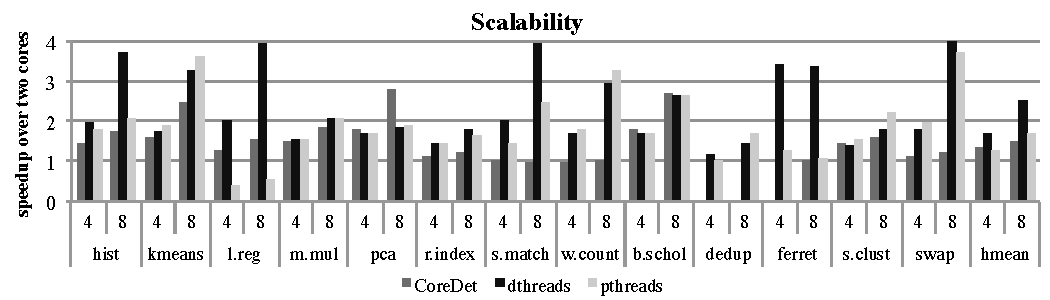
\includegraphics[width=6in]{dthreads/figure/scalability-figure}
\caption{Speedup of eight cores versus two cores (higher is better).  When possible to control with command line options, the number of threads was matched to the number of cores enabled.\label{fig:scalability}}
}
\end{figure}

To measure the scalability cost of running \dthreads{}, we ran two benchmark suite (excluding \texttt{canneal}) on the same machine with eight cores and again with two cores enabled.  Whenever possible without source code modifications, the number of threads was matched to the number of CPUs enabled.  We have found that \dthreads{} scales at least as well as \pthreads{} for 9 of 13 benchmarks, and scales as well or better than CoreDet for all but one benchmark where \dthreads{} outperforms CoreDet by 2x.  Detailed results of this experiment are presented in Figure~\ref{fig:scalability} and discussed below.

\texttt{canneal} was excluded from the scalability experiment because this benchmark does more work when more threads are present, making the performance comparison between eight and two threads unfair.  \dthreads{} hurts scalability relative to \pthreads{} for four of the benchmarks: \texttt{kmeans}, \texttt{word\_count}, \texttt{dedup}, and \texttt{streamcluster} although only marginally in most cases.  In all of these cases, \dthreads{} scales better than CoreDet.

\dthreads{} is able to match the scalability of \pthreads{} for three benchmarks: \texttt{matrix\_multiply}, \texttt{pca}, and \texttt{blackscholes}.  With \dthreads{}, scalability actually \emph{improves} over \pthreads{} for 6 out of 13 benchmarks: \texttt{histogram}, \texttt{linear\_regression}, \texttt{reverse\_index}, \texttt{string\_match}, \texttt{ferret}, and \texttt{swaptions}.

